%!TEX root = ../thesis.tex
%*******************************************************************************
%****************************** Fifth Chapter *********************************
%*******************************************************************************

\chapter{Population-scale differentiation of iPSCs to a neuronal fate}

The study described in chapter 4 acted as a proof of principle study where we demonstrated that pooling..

In this second study, we scale up .. and apply similar principles to a much longer and more complex differentiation protocol, considering iPSCs differentiating towards a midbrain neuronal fate.\\

First, the use of the droplet-based scRNA-seq technology allows us to assay a much larger number of cells providing an overview of the plethora of brain cell types generated by this protocol. 
Moreover, the larger number of cell lines included and the longer protocol allows us to dive deeper into the differences across lines in efficiency to differentiate, and allows us to start exploring possible causes.
Finally, the closer resemblance of the differentiated cells to primary tissues allows to start looking into the effects of disease-associated variants onto specific cell types and across development. \\

Briefly, the dataset we describe in this chapter is genome-wide single cell RNA-sequencing profiling of over one Million differentiating iPS cells collected from cell lines from 215 healthy donors. 
Data is collected at three maturation stages following differentiation to midbrain dopaminergic neurons: progenitor-like state (day11), young neurons (day30), and more mature neurons (day52). 
Additionally, just before the latest time point half of the cells were stimulated with rotenone, to simulate oxidative stress. 

\newpage

\begin{Comment2}

\hspace{-3mm}\textbf{Contributions} This work is the result of a collaboration between the Stegle, Merkle, Marioni and Gaffney labs, and was funded by Open Targets 
(https://www.opentargets.org).
The data was generated by Dan Gaffney’s lab at the Wellcome Trust Sanger Institute, and the experiments were led by Julie Jerber, who also contributed to the interpretation of the results. 
The statistical methods and analyses described in this chapter were co-supervised by Dan Gaffney and Oliver Stegle. 
Daniel Seaton processed the data and performed \gls{qc}. 
Daniel and I developed and implemented the statistical methods under the supervision of Oliver Stegle and Dan Gaffney with some input from Florian Merkle, John Marioni and Natsuhiko Kumasaka.
In particular, Natsuhiko performed the colocalisation analysis.
The code for processing, analysing and plotting the data is open source and freely accessible here: https://github.com/single-cell-genetics/singlecell\_neuroseq\_paper.
Julie Jerber, Daniel Seaton, Florian Merkle, Dan Gaffney, Oliver Stegle and I wrote the manuscript, with input from Natsuhiko Kumasaka and John Marioni.
A preprint \cite{jerber2020population} can be found on biorxiv: https://www.biorxiv.org/content/10.1101/2020.05.21.103820v1, as:\\

Julie Jerber*, Daniel D. Seaton*, Anna S.E. Cuomo*, Natsuhiko Kumasaka, James Haldane, Juliette Steer, M Patel, D Pearce, M Andersson, Marc Jan Bonder, Ed Mountjoy, Maya Ghoussaini, Madeline A. Lancaster, the HipSci Consortium, John C. Marioni, Florian T. Merkle, Oliver Stegle, Daniel J. Gaffney. Population-scale single-cell RNA-seq profiling across dopaminergic neuron differentiation, 2020 (* equal contributions).

\end{Comment2}

\newpage

\section{Introduction}

As discussed, genetic variation can significantly alter cell function, for example by altering gene expression. 
Human iPSCs are a promising cellular model for assessing the cellular consequences of human genetic variation across different lineages, developmental states and cell types. 
In particular, human iPSCs facilitate the study of developmental time points and stimulation conditions that would be challenging to obtain \textit{in vivo}. 
The creation of cell banks containing hundreds of iPSC lines \cite{kilpinen2017common} provides an exciting opportunity to carry out population-scale studies \textit{in vitro} \cite{cuomo2020single, strober2019dynamic, schwartzentruber2018molecular, alasoo2018shared}.
However, differentiating iPSCs is expensive and labour-intensive, and differentiation experiments are difficult to compare due to substantial batch variation. 
Thus, studies of more than a handful of lines remain a significant challenge.
Furthermore, most iPSC differentiation protocols produce a heterogenous population of cells of which the target cell type is a subset \cite{d2019vitro, banovich2018impact, volpato2018reproducibility, nguyen2018single}. 
This variability in differentiation outcomes hinders efforts to dissect the genetic contributions to cellular phenotypes.\\

Single cell sequencing has enabled “multiplexed” experimental designs, where cells from multiple donors are pooled together \cite{cuomo2020single, nguyen2018single}. 
Pooling improves throughput and allows experimental variability between differentiation batches to be rigorously controlled, by enabling cell type heterogeneity to be accounted for in downstream analysis. 
To date, multiplexed experimental designs have only been applied to short differentiation protocols (over a period of days), that generate cells corresponding to very early stages of development, and have not captured developmental progression toward a mature cell fate. 
Population-scale pooling during long-term differentiation offers the opportunity to examine the effect of common genetic variants on gene expression in each cell population produced over neural development, providing a foundation for future mechanistic studies.

Here, we develop and apply a multiplexing strategy to profile the differentiation and maturation of more than two hundred iPSC lines derived from gls{hipsci} towards a midbrain neural fate, including dopaminergic neurons (DA). 
DA are involved in motor function and other cognitive processes and play key roles in neurological disorders, including Parkinson’s Disease (PD)\footnote{Parkinson’s disease (PD) is a progressive neurodegenerative disorder, characterized by the loss of midbrain DA neurons. 
These neurons control motor behavior, and, as they degenerate, they result in several motor features of the disease, such as bradykinesia, rigidity, resting tremor, gait disturbances and postural instability \cite{lees2009parkinsons}.} \cite{osborn2017seq, stoddard2020stem}. 
To study how these cells differentiate, and how genetic background could influence differentiation, we employed a well-established protocol \cite{kriks2011dopamine} and collected cells at three maturation stages (progenitor-like, young neurons, and more mature neurons), covering 52 days of differentiation. 
We additionally exposed cells on day 51 to rotenone, to explore how genetic variation shapes the neuronal response to oxidative stress. 
Using this system, we create the first map of \gls{eqtl} at multiple stages of human neuronal differentiation, and identify nearly 500 novel trait / \gls{eqtl} colocalisations. 
Using estimates of cell population composition based on single cell RNA-seq, we demonstrate that a strong, cell intrinsic-differentiation bias affects a significant proportion of \gls{ipsc} lines, such that approximately 25\% reproducibly fail to produce any neuronal cells.\\

longer iPSC differentiation protocol

relevant for cell therapy (dopaminergic neurons and PD)

different 

\section{Single cell map of iPSCs neuronal differentiation}

\subsection{Experimental strategy and data generation}

215 iPSC lines from HipSci were cultured ...

24h after plating, neuronal differentiation of the pooled lines to a midbrain lineage was performed as described by Kriks \textit{et al} \cite{kriks2011dopamine}.

Maybe briefly add what molecules are added and to mimick what.
Day11 should correspond to week 5 which is the beginning of neurogenesis \textit{in vivo}. 

Each pool contained cells from between 7 to 24 lines.

Droplet based scRNA-Seq was performed using the 10X Genomics™ technology \cite{zheng2017massively}

\begin{figure}[h]
\centering
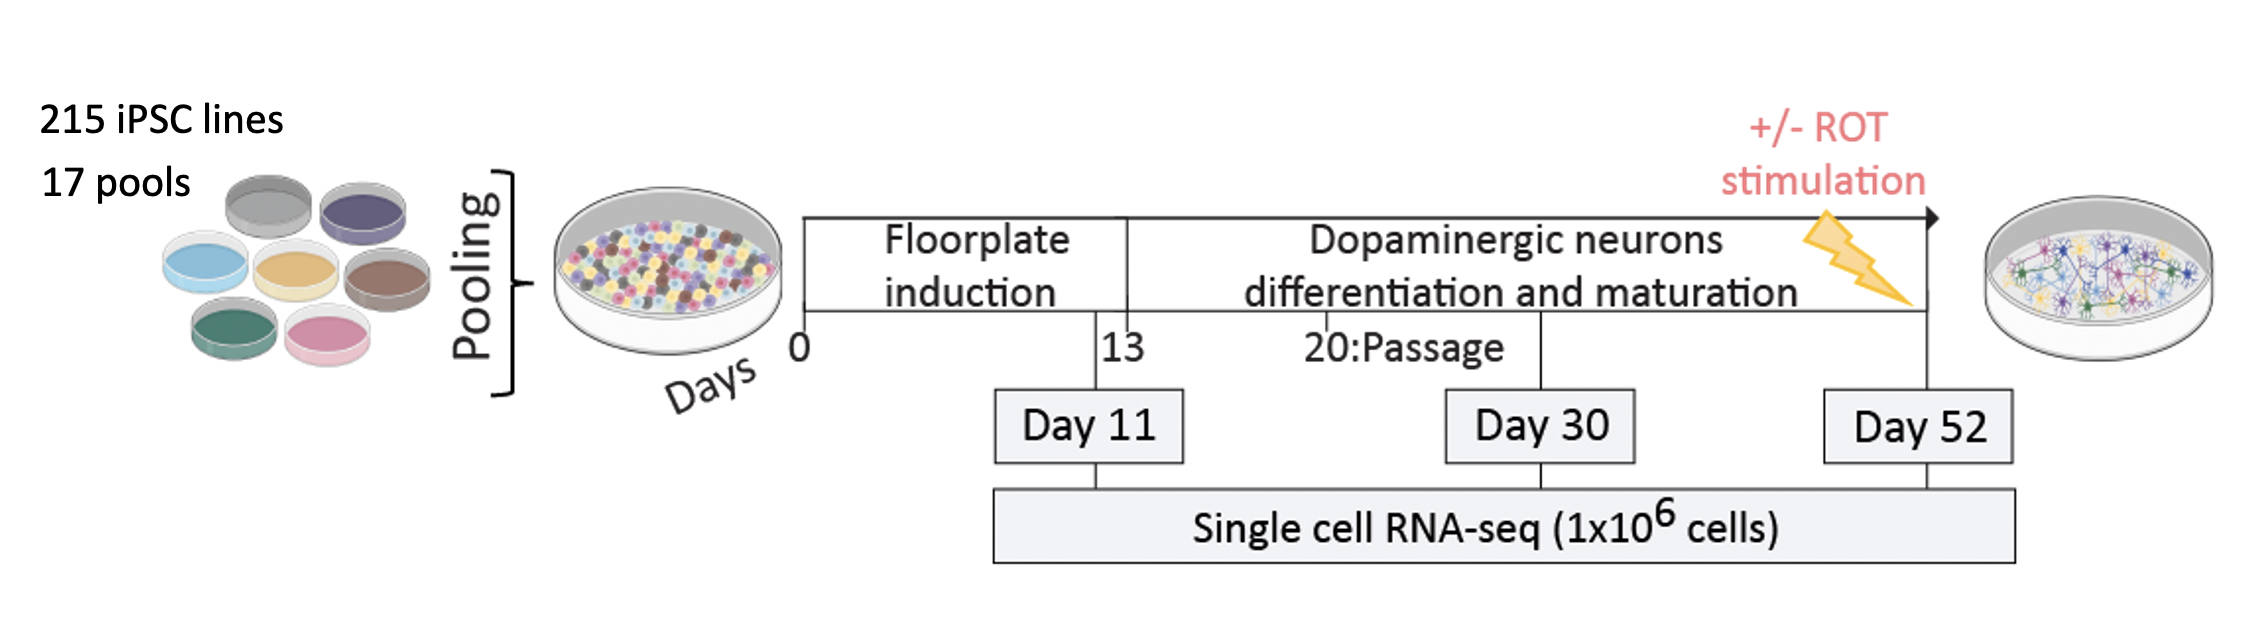
\includegraphics[width=16cm]{Chapter5/Fig/neuroseq_experimental_design.png}
\caption[\textbf{Experimental Design}]{\textbf{Experimental Design}.\\
}
\label{fig:neuroseq_experimental_design}
\end{figure}

\subsection{Data processing and QC}

For each of 19 pooled experiments, donors (i.e. cell lines) were demultiplexed using demuxlet \cite{kang2018multiplexed}, using genotypes of common (MAF>1\%) exonic variants available from the HipSci bank, and a doublet prior of 0.05. 
Only single cells with successful donor identification were retained for further analysis. 
This step filtered out two types of droplet: those containing two or more cells from different individuals, and those containing no cells, but that contained a mixture of free-floating RNA and had therefore passed the CellRanger UMI filter (above).




\section{Data overview}

We selected 215 iPSC lines derived from healthy donors by the HipSci project \cite{kilpinen2017common} for differentiation towards a midbrain cell fate, including dopaminergic neurons 12 \cite{kriks2011dopamine}. 
Differentiation experiments were multiplexed using pools containing between 7 and 24 cell lines per experiment. 
Immunochemistry confirmed that cells from both pooled and conventional differentiation of individual lines expressed protein markers associated with patterning of DA (LMX1A, FOXA2 and TH). 
To capture transcriptional changes during neurogenesis and neuronal maturation, we performed single cell RNA sequencing (scRNA-seq) of cells captured at day 11 (D11, midbrain floorplate progenitors), day 30 (D30, young post-mitotic midbrain neurons) and day 52 (D52, more mature midbrain neurons). 
To mimic an oxidative stress condition, we also profiled day 52 neurons upon exposure to a sub-lethal dose of rotenone (ROT, 0.1 μM; 24 h) a chemical stressor that preferentially leads to DA death in models of PD \cite{xiong2012mitochondrial}.

\subsection{Normalisation, dimensionality reduction, and clustering}

After QC, we obtained a total of 1,027,401 cells across 19 cell pools 14 and four conditions. 
The cell line of origin for each cell was inferred from single cell RNA-seq read data using known genotypes made available by the HipSci consortium (using demuxlet, \cite{kang2018multiplexed}). Adjustment for experimental batch effects using Harmony \cite{korsunsky2019fast} followed by Louvain clustering \cite{blondel2008fast} identified a total of 26 clusters (6, 7 and 13 clusters respectively at D11, D30, D52). 
These clusters were then assigned to cell types by testing for enrichments of 48 literature-curated marker genes of major brain cell types.\\

Among these, we identified six dominant cell types that were making up at least 10\% of the cells at any time point. 
These included two main cell type populations at day 11: proliferating and non-proliferating midbrain floorplate progenitors (both expressing \textit{LMX1A, FOXA2} and expressing \textit{MIK67, TOP2A} when proliferating \cite{la2016molecular}). 
At days 30 and 52, four additional dominant cell types were identified. Two of these additional cell types appeared neuronal and two were non-neuronal (characterised by expression and lack of the pan-neuronal markers \textit{SNAP25} and \textit{SYT1} respectively ). 
The two neuronal populations could be further divided into midbrain dopaminergic neurons, which expressed \textit{NR4A2, PBX1, TMCC3} \cite{la2016molecular, park2006acquisition, ramonet2012park9} and serotonergic neurons (Sert), which expressed \textit{TPH1, TPH2, GATA2} \cite{cummings2019serotonergic}. 
The two non-neuronal cell types corresponded to ependymal-like cells, detected both at days 30 and 52 (Ependymal 1 \cite{campbell2017molecular}) and astrocyte-like cells, unique to day 52 (Astrocyte-like \cite{sloan2017human, zhang2016purification}). 
We also identified a neuroblast population, specific to day 11 (4\% of all cells at day 11) expressing pro-neuronal genes (\textit{NEUROD1, NEUROG2, NHLH1} \cite{bertrand2002proneural, lacomme2012neurog2}) and an additional neuronal population (expressing \textit{SNAP25} and \textit{SYT1}) that could not be assigned to a specific neuronal identity (Unknown neurons 1, present at Day 30 and Day 52 at around 7\%). 
Finally, we identified four additional rare cell types (<2\% of cells sampled at any time point), including a second ependymal-like population (Ependymal 2), a proliferating neuronal serotonergic population (Prolif. Serotonergic neurons), and two additional neuronal populations which could not be annotated unambiguously (Unknown neurons 2, Unknown neurons 3).\\

UMAP projection of cells collected across all time points, stimuli and lines revealed broad co-clustering of cell types, but with noticeable differences between time points and stimuli. 
We observed substantial variation in the cell type proportions across time points
and stimuli. 
For example, the proportion of DA upon ROT stimulation was significantly reduced (30\% reduction upon stimulation, Fisher’s exact test, p value=$2.2x10^{-16}$ ), consistent with previous observations that dopaminergic neurons are most affected by apoptosis due to oxidative stress \cite{sherer2003mechanism, knonagel1992autologous, cannon2009highly}.
Collectively, our population-scale scRNA-seq analysis revealed a surprisingly diverse repertoire of cell types, enabling study of both cell line differentiation propensity and the identification of genetic variants that act in a cell type-specific manner.

\section{Line-to-line variation in differentiation efficiency}

iPSC differentiation protocols are highly variable but the biological basis for this remains largely obscure, which hinders efforts to rationally select cell lines for specific applications \cite{d2019association, volpato2018reproducibility}. 
We found substantial variation in the proportions of different cell types produced by different iPSC cell lines at each time point. 
Using principal component analysis of cell type fractions per cell line and pool, we identified the proportion of midbrain neurons (DA and Sert) on day 52 as the largest axis of variation (PC1, 47\% variance). 
Since DA and Sert cells are derived from similar progenitor populations \textit{in vivo}, it is not surprising that both populations are observed in our differentiation experiment 31 \cite{ye1998fgf}. 
This motivated us to estimate “differentiation efficiency” for each iPSC line, defined as the sum of the proportions of DA and Sert cells produced on day 52. 
We assessed the reproducibility of this measure of differentiation efficiency using data from 35 lines that were differentiated twice, in two different pools. 
Importantly, we found that iPSC line differentiation efficiency defined in this way was highly reproducible between different pools (Pearson R=0.75; p=$2x10^{-6}$).\\

Given the robustness of these results, we wondered if they were generalisable to other neuronal differentiation approaches. We therefore differentiated a pool of 18 lines (pool 4) into cerebral organoids for 113 days 32 \cite{lancaster2017guided} and profiled the resulting cell populations using scRNA-seq (11,445 cells). 
Remarkably, we found that the proportion of brain cell types (all neural, glial, and neural progenitor cells) produced by each line in the cerebral organoids was strongly correlated with differentiation efficiency as estimated from the dopaminergic differentiation (R=0.94; p=$2x10^{-5}$; n=12). 
Taken together, these results strongly suggest that variation in iPSC neural differentiation efficiencies arise primarily due to cell-intrinsic factors. 
Furthermore, the consistency of differentiation efficiency suggests these properties extend to neuronal differentiation more generally.

\section{iPSC expression can predict differentiation efficiency}

Motivated by the reproducibility of differentiation outcomes across multiple independent pools, we tested for associations between differentiation efficiency and other experimental and biological factors, but found no or weak associations with cell line passage number (p=0.77), donor sex (p=0.008), chromosome X activation status (p=0.01), or PluriTest scores \cite{muller2011bioinformatic} (p=0.01).\\

Next, we assessed whether differentiation efficiency was associated with particular patterns of gene expression in undifferentiated iPSCs. 
Using data from independent bulk RNA-seq data available for a subset of 184 iPSC lines included in this study \cite{kilpinen2017common, bonder2019systematic} we identified significant associations with differentiation efficiency for 2,045 genes (983 positive and 1,062 negative associations; F-test, FDR < 5\%). 
Notably, when defining poor differentiation as a binary outcome (differentiation efficiency < 0.2), genome-wide gene expression profiles in undifferentiated iPSCs were able to predict differentiation outcomes (logistic regression; 100\% precision at 35\% recall assessed using cross-validation). 
This result was robust to alternative thresholds for defining poor differentiation outcomes. Using this model, we generated predicted scores for all 812 HipSci lines with bulk RNA-seq data.
This analysis indicated that a substantial fraction of lines in the HipSci resource (26\%) were predicted to produce < 20\% neuronal cells under the differentiation conditions we tested.
Furthermore, we tested whether the same experimental and biological factors previously associated with differentiation efficiency replicated in this larger sample and found consistent results.
Finally, we also observed substantial variation in predicted outcomes of different lines from the same donor, suggesting that donor genetic background is unlikely to play a role in driving differentiation biases.\\

Next, since iPSC cultures are heterogeneous, we hypothesised that the identified predictive gene signatures might arise from varying proportions of an iPSC subpopulation. 
To test this hypothesis, we re-analysed scRNA-seq data from 112 iPSC lines that were assayed previously under iPSC culture conditions similar to those used here 2 
\cite{cuomo2020single}, 45 of which were also included in this study). 
We identified 5 clusters, all but one of which expressed similarly high levels of core pluripotency markers (\textit{NANOG, SOX2, POU5F1}). 
We found that genes whose expression predicted poor differentiation (e.g \textit{UTF1}) were highly enriched in one of those clusters (cluster 2), while genes whose expression were predictive of successful differentiation (\textit{TAC3}), were downregulated in cluster 2 relative to the remaining iPSC clusters. 
In comparison, other cell clusters did not show such equivalent enrichment in differentiation marker genes.\\

As a direct confirmation of this hypothesis, we also tested for and confirmed an association between the fraction of cells in cluster 2 and differentiation efficiency for each cell line (Pearson R=-0.76, p=$2.05x10^{-9}$). 
We used additional data from 2 to assess the consistency of the fraction of cluster 2 cells across replication experiments, finding high concordance (Pearson R=0.9; n=23).
Using the known relationship between iPSC bulk RNA-seq and the proportion of cluster 2 cells, we predicted this proportion for 182 cell lines included in our differentiation experiments, and confirmed the negative correlation with differentiation efficiency (Pearson R=-0.49; p=3x10 -12). 
Finally, we also analysed an additional scRNA-seq dataset from iPSCs derived from Lymphoblastoid Cell Lines \cite{sarkar2019discovery} (LCLs). 
Using our single cell analysis pipeline, we also identified a cluster of cells with a concordant expression profile to cluster 2. 
Taken together, these results provide further evidence that a subpopulation of iPS cells with poor differentiation capability is consistently detected across different human iPSCs banks, and that this bias can be robustly predicted using expression markers at the iPSC stage. 
Importantly, despite the variability in differentiation efficiency, our single-cell sequencing approach enabled us to examine multiple disease-relevant cell populations for many cell lines. Correlating changes in gene expression with common genetic variants associated with various traits in GWAS could provide insights into disease mechanisms.

\section{eQTL mapping in neuronal cell types}

Next, we mapped eQTL in the cell types defined above.
Here our focus was on understanding how individual-to-individual genetic variation influenced gene expression across these cell types during differentiation and in response to stimulation.
Specifically, we mapped \textit{cis} expression quantitative trait loci (eQTL) separately for each of the 14 distinct cell populations that corresponds to the profiled “cell type”-“condition” contexts (fig.). 
eQTL were mapped by calculating aggregate expression levels for each donor, considering common gene-proximal variants (MAF>0.05, plus or minus 250 kb around genes; Methods). 
Variability in differentiation efficiency between lines resulted in substantial differences in the number of cells collected for each donor (Supplementary Fig. 8a), affecting accuracy of the estimates of aggregated expression. 
To account for this source of noise, we adapted commonly used eQTL mapping strategies2 based on linear mixed models (LMMs) by incorporating an additional variance component into the model (Methods). 
This approach greatly increased the power to map eQTL, resulting in a total of 4,087 genes with at least one eQTL in any of the contexts (hereafter “eGene”, FDR < 5\%, Fig. 4a, Supplementary Fig. 8b, Supplementary Table 7).


In Chapter 4 we have focused on reproducing standard "mean-level" expression level eQTL mapping using scRNA-seq, where the phenotype of interest is expression abundance within a homogeneous population of cells.
We can call such efforts "pseudo-bulk" approaches, where we are essentially replicating bulk-like expression values and performing the eQTL test adapting approaches used for traditional eQTL mapping using bulk RNA-seq. 
In the applications we and others have described \cite{van2018single,cuomo2020single}, the value of using scRNA-seq lies in the fact that we are able to, within a single experiment, unbiasedly define and assess multiple different cell types, whilst retaining a single cell resolution.\\



\section{Discussion}

disease relevance

protocol efficiency

cell type composition - joint model